\documentclass{article}
\usepackage{graphicx}
\usepackage{listings}
\usepackage{xcolor}
\usepackage{wrapfig}
\usepackage{multicol}
\usepackage{float}
\usepackage{booktabs}

\colorlet{punct}{red!60!black}
\definecolor{background}{HTML}{EEEEEE}
\definecolor{delim}{RGB}{20,105,176}
\colorlet{numb}{magenta!60!black}

\lstdefinelanguage{json}{
    basicstyle=\fontsize{6}{5}\ttfamily,
    showstringspaces=false,
    breaklines=true,
    literate=
     *{0}{{{\color{numb}0}}}{1}
      {1}{{{\color{numb}1}}}{1}
      {2}{{{\color{numb}2}}}{1}
      {3}{{{\color{numb}3}}}{1}
      {4}{{{\color{numb}4}}}{1}
      {5}{{{\color{numb}5}}}{1}
      {6}{{{\color{numb}6}}}{1}
      {7}{{{\color{numb}7}}}{1}
      {8}{{{\color{numb}8}}}{1}
      {9}{{{\color{numb}9}}}{1}
      {:}{{{\color{punct}{:}}}}{1}
      {,}{{{\color{punct}{,}}}}{1}
      {\{}{{{\color{delim}{\{}}}}{1}
      {\}}{{{\color{delim}{\}}}}}{1}
      {[}{{{\color{delim}{[}}}}{1}
      {]}{{{\color{delim}{]}}}}{1},
}

\DeclareFontFamily{\encodingdefault}{\ttdefault}{\hyphenchar\font=`\/}


\begin{document}
\begin{titlepage}
  \begin{center}
    
\includegraphics[width=10cm, height=10cm, keepaspectratio]{epfl}
    \vspace*{0.5cm}

    \Huge
    \textbf{Course Recommendation System}

    \vspace{5cm}

    \Large
    Center for Digital Education\\
    \vspace{1cm}
    Romain \textsc{Choukroun}\\

    \vspace{2.3cm}
      \begin{flushleft}
      \textbf{Supervisors}\\
      Prof. Patrick Jermann, Francisco Pinto, Kshitij Sharma
      \end{flushleft}

    \vspace{0.24cm}
    \large
    January 2018

    \end{center}
\end{titlepage}

\newpage
\tableofcontents

\newpage
\section{Abstract}
    Recommender systems have been flourishing the past few years, and with the amount of data lying untouched these days, there is much to do. The main idea behind a recommender system is, to combine the knowledge and empathy of a human being with the sheer amount of data contained in a database in order to recommend multiple things to people.
    \\As humans, we would have a hard time to recommend items to different people each with their own set of preferences and wishes, and what about a hundred people, a million ?
    \\Clearly, fitting the requirements of such a system is impossible for human beings, however, we are able to teach our own machines to do so, efficiently. There are a ton of ways to create such a system, from collaborative filtering to similarity measures, and even graph-based methods like clustering.
    \\There is a need for recommender systems in society and universities, for many different things, such as courses, which is what we're going to focus on in this paper.
    \\What happens when you set foot in a university to study any subject is that most of the time you do not know which courses to pick out of all the possibilities. We want to solve this problem, and find a way to recommend courses to someone new or a current student advancing to the next year.

\newpage
\section{Introduction}
    \subsection{Motivation}
        The average student, usually, has a rough idea of what they want to study during their time at university, but they might not know enough people to get the best recommendations concerning courses.
        \\Let's take a look at a concrete example, drawn from countless reports out of students from EPFL. Let's say the student is a master student in computer science, and wants to work on data science. Well it turns out that there are a ton of courses in the computer science masters cursus related to data science to choose from right off the bat. And some of the best courses on the subject come from other faculties such as Electrical Engineering, Life Sciences or even Microengineering.
        \\This makes it so hard to stumble upon the right ones. The phenomenon is known to exist in most faculties, namely the ones where students can build their study plan as they wish, with a lot of flexibility.
    \subsection{Recommender System}
        The idea behind the system we wrote is to recommend courses to a student who only has to provide the list of courses (s)he already took or knows they will take, and the system will simply return the top-10 courses it thinks that the person is most likely to enjoy.
        \\As the project is mainly a proof of concept, it can be greatly improved, we were not shooting for the state of the art recommender system, but more towards an accurate and simple system that makes sense, opposed to a blackbox. That being said, it has a really good accuracy as we will see, and could be used out of the box, university-wide.
        \\Although, it really is important to note that the system focuses only on master level courses as study plans for the bachelor degree is mostly the same within each section. We want to be able to recommend courses to people who actually have quite a bit of freedom into choosing their curriculum, which mostly happens at master level.

\newpage
\section{Data Handling}
    \subsection{Available Data}
        A lot of data was made available to support the project: the school provided a database with the courses registrations and grade correlations for a total span of 15 years. So here is what the registrations table looks like:

\begin{flushleft}
\scalebox{0.7}{
\begin{tabular}{lllllll}
\toprule
{} & PedagogicalCode &    StudyDomain &      UnitName &                                      SubjectName & CourseCode &   YearName \\
PersonID  &                 &                &               &                                                  &            &            \\
\midrule
29123807  &             MA1 &   Architecture &  Informatique &                              Théorie de l'espace &     AR-461 &  2012-2013 \\
109679682 &             MA3 &  Life sciences &  Informatique &  Cellular biology &    BIO-105 &  2008-2009 \\
2416702   &             MA3 &  Life sciences &  Informatique &  Cellular biology &    BIO-105 &  2008-2009 \\
40908413  &             MA3 &  Life sciences &  Informatique &  Cellular biology &    BIO-105 &  2008-2009 \\
82030336  &             MA3 &  Life sciences &  Informatique &  Cellular biology &    BIO-105 &  2008-2009 \\
\bottomrule
\end{tabular}}
\end{flushleft}
        Each line is a registration from a student into a course, we have a ton of other information to leverage in addition to that. The data is quite sparse, we have $1823$ courses and $7999$ students for $136962$ registrations which means that the matrix will be $99\%$ sparse. The most important columns are the PersonID and the SubjectID which represent the student and the course. In addition, we get the study domain of the course as well as the section name of the student. So, we can differentiate inbetween sections to perfect the recommendation (Architecture students are less likely to pick Life Science courses for example). The year in which the registration was made is also available, which we should be able to leverage using time series in the near future. There are still a few bits of the table that we cannot apparently leverage, such as the code of the course or the unit and the pedagocial code, so we kept the data to simply have more information about registrations in case we need it. We also have the correlation inbetween the grades of a student in one course and in another, both when the first course was taken before the second one, and in the reverse case. Now let's take a look at how we transformed the data to create exploitable features.

    \newpage
    \subsection{Features}
        For the correlations, we only kept the mean of both correlations, to then normalize and transform them into probabilistic distributions such that for a single course, adding its correlations with regard to the other ones sums up to $1$. These correlations are now more of a score of some sort describing how the distribution of grades inbetween two courses relates to one anoter. And here is an excerpt of what the data looks like:
\begin{flushleft}
\scalebox{0.7}{
\begin{tabular}{lrrr}
\toprule
{} &  Advanced computer graphics &  Advanced databases &  Algorithms \\
sub2\_name                             &                             &                     &             \\
\midrule
Advanced algorithms                   &                    0.007003 &            0.006472 &    0.006323 \\
Advanced computer architecture        &                    0.006327 &            0.006318 &    0.006323 \\
Advanced cryptography                 &                    0.006327 &            0.006318 &    0.006323 \\
Advanced theoretical computer science &                    0.006327 &            0.006318 &    0.006323 \\
Algebra                               &                    0.006327 &            0.006318 &    0.006323 \\
Algorithms                            &                    0.006327 &            0.006318 &    0.006323 \\
Algèbre                               &                    0.006327 &            0.006318 &    0.006323 \\
Analyse I                             &                    0.006327 &            0.006318 &    0.006323 \\
Analyse II                            &                    0.006327 &            0.006318 &    0.006323 \\
Analyse III                           &                    0.006327 &            0.006318 &    0.006323 \\
\bottomrule
\end{tabular}}
\end{flushleft}
        The bulk of the work stands on the registrations to courses, and here we decided to do something really simple, using all of the courses at our disposal as well as all of the registrations, we created a binary matrix of students vs courses where $1$ means that the student took the course and $0$ means that the (s)he did not. So here is how it looks like:
\begin{flushleft}
\scalebox{0.7}{
\begin{tabular}{lrrr}
\toprule
SubjectName &  Advanced analysis II &  Advanced compiler construction &  Advanced computer architecture \\
PersonID &                       &                                 &                                 \\
\midrule
2412404  &                     0 &                               0 &                               0 \\
2414145  &                     0 &                               0 &                               0 \\
2416702  &                     0 &                               0 &                               0 \\
2436004  &                     0 &                               0 &                               0 \\
2480734  &                     0 &                               0 &                               1 \\
2501514  &                     0 &                               0 &                               0 \\
2501538  &                     0 &                               0 &                               0 \\
2505593  &                     0 &                               0 &                               0 \\
2523797  &                     0 &                               0 &                               0 \\
2526528  &                     0 &                               1 &                               0 \\
\bottomrule
\end{tabular}}
\end{flushleft}
        Finally the last feature we decided to leverage was co-enrolments. The idea here is that the sheer amount of people taking two courses in their study plan means it's quite likely that both of them are linked in some fashion, and the more people take them, the higher the probability that they are, in fact, linked. Once again we normalized them, and transformed each of them to density distributions, hence every row of the matrix sums up to 1. Here's how it looks:
\begin{flushleft}
\scalebox{0.7}{
\begin{tabular}{lrrr}
\toprule
SubjectName &  Advanced analysis II &  Advanced compiler const. &  Advanced computer arch. \\
SubjectName                    &                       &                                 &                                 \\
\midrule
Accounting for finance         &              0.000000 &                        0.000000 &                        0.000000 \\
Advanced algorithms            &              0.000000 &                        0.048826 &                        0.024227 \\
Advanced analysis I            &              0.090909 &                        0.000000 &                        0.000000 \\
Advanced analysis II           &              0.000000 &                        0.000000 &                        0.000000 \\
Advanced compiler const.       &              0.000000 &                        0.000000 &                        0.016708 \\
Advanced computer architecture &              0.000000 &                        0.018779 &                        0.000000 \\
Advanced computer graphics     &              0.000000 &                        0.017840 &                        0.017544 \\
\bottomrule
\end{tabular}}
\end{flushleft}

    \newpage
    \subsection{Data Storing}
        All of the data aforementioned are queries from a database located in the CEDE\cite{cede} lab, and as long as the tables do not change, the code and notebooks provided will be able to run like a charm, simply fill in your credentials in the credentials.ini file. There is also the possibility to download all of the necessary tables in a local folder, if the need to work offline comes along. To learn how to do so, checkout the README.

\section{Setup}
    The tool has been written exclusively in python and uses a few libraries such as keras\cite{keras}, numpy and pandas. Python was an obvious choice and is quite standard for exploratory analysis, the other libraries are pretty much standard in the same regard, as to keras\cite{keras}, we chose it for the simplicity of its syntax since we have quite a simple neural network.
    \\Now let's take a look at the setup for our recommender system in terms of what we feed it, what we get in return and how to measure if it's a good recommendation or not.

    \subsection{Input and Output}
        We decided that the system should be as simple as possible to use, which means that anyone, even someone who is not from EPFL should be able to make use of it. In that spirit, the input will only be a list of courses. Courses that the student either took in previous years, or courses that are of the highest interest to him/her, the idea being that if you know you will like some courses, we can still recommend similar courses that you will most likely enjoy too.
        \\The algorithm then returns a small list of courses recommended for your profile.

    \subsection{Metrics}
        But how do we know that we have good recommendations ? There are a few metrics we could use. First we define the precision as the percentage of recommended courses that were taken by the student, we also define the recall as the percentage of courses picked by the student which were also recommended.
        \\However the most important one is the top-N success rate which is the probability that the student picks at least one out of the N recommended courses. So we aim towards a decent precision/recall, but most importantly we want to maximize the top-N success rate as we want to maximize our chances that the student will pick at least one course from the recommendations.

\newpage
\section{Exploration}
    We are going to list here all of the collaborative filtering techniques that were tried but did not make the final cut as they were outperformed by another one. This is the main reason why we will go quite quickly over them to focus on the final pipeline in the next section.

    \subsection{Jaccard Similarity}
        Here the idea is to apply the oldest trick in the book, collaborative filtering, but using the Jaccard similarity\cite{jaccard} to compare vectors. We started out thinking cosine-similarity would be a good one to use but it simply makes more sense to treat recommendations and taken courses as two binary vectors, hence the Jaccard similarity\cite{jaccard}. We computedit the following way:
        \begin{center}
        $J(\mathbf{x}, \mathbf{y}) = \frac{\sum_i \min(x_i, y_i)}{\sum_i \max(x_i, y_i)}$
        \end{center}

    \subsection{Jensen-Shannon Divergence}
        Exactly like the previous case, we used a Jensen-Shannon divergence\cite{jensen} assuming that each student is represented by its own probability distribution, meaning that we assume similar students should be samples out of the same underlying distribution. Following this reasoning, it made sense to try the Jensen-Shannon divergence\cite{jensen} which we computed the following way:
        \begin{center}
        ${\rm JSD}(P \parallel Q)= \frac{1}{2}D(P \parallel M)+\frac{1}{2}D(Q \parallel M)$
        \end{center}

    \subsection{KNN}
        We also tried a graph-based approach with K-Nearest neighbors, which gave out poor results which are mot likely due to the sub-par embedding of the data for a graph context. However it would seem logical that similar students be clustered together in a high dimensional plane, with the clusters being representative of underlying concepts such as sub-domains of each faculty. This surely needs more work, however, we did not pursue a graph-based approach this time.

    \subsection{NMF}
        Once again, we tried a collaborative filtering approach using Non-negative Matrix Factorization. There is not much to say about NMF as it's quite standard and in our case did not work well.

    \subsection{Co-Clustering}
        Exactly the same as for KNN, we're lacking a graph-based representation to be able to apply co-clustering hence we did not get any significant results.

\section{Pipeline}
    Now, let's dig into the current pipeline used to recommend courses. As the subject is trendy these days, we too implemented a simple neural network that actually did a wonderful job.

    \subsection{Collaborative Denoising Auto-Encoder}
        The neural network is a Collaborative Denoising Auto-Encoder\cite{cdae}, and looks like this:
\\\begin{figure}[h]
\centering
\scalebox{0.5}{
  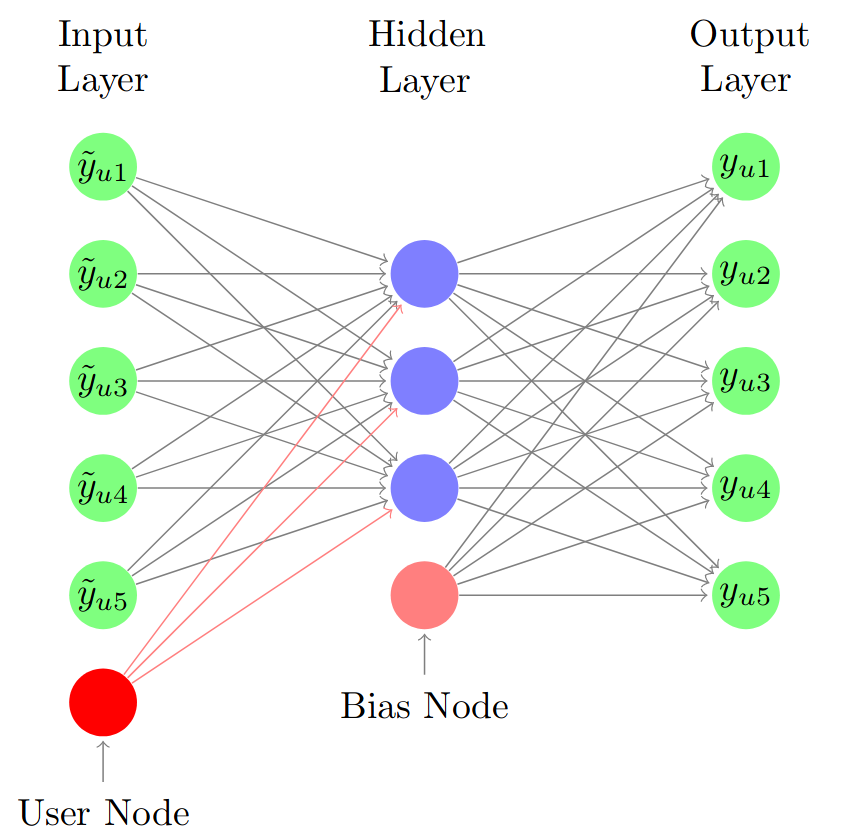
\includegraphics[width=\linewidth]{../figures/cdae_layers.png}}
  \caption{Collaborative Denoising Auto-Encoder}
  \label{fig:cdae_layers}
\end{figure}
        \\We implemented it using keras, following quite the same implementation as the one found in henry0312's github\cite{cdaegithub}. As the network is simple, it was quick to implement and optimize. A binary vector of enrolments-by-user is fed into the network to then get out a confidence score for each pair of student/course. The optimized parameters for the network are the following: we have $27$ nodes in the hidden layer and a dropout rate of $99.8\%$ using ReLU as a hidden activation function, with the final layer activated by a sigmoid. Now onto the interesting part, recommending courses.

    \newpage
    \subsection{Recommendations}
        The recommendations are obtained by combining three parts: the neural network, the matrix of correlations, and the matrix of co-occurrences. Each of them returns a confidence score between $0$ and $1$ by student/course combo, Which means that to get the final score we simply multiply them together and sort them from largest to smallest. The largest confidence score for a student designates the course that they will be most likely to pick.
        \\To maximize the results, we ask the student his/her section so that we can restrain the choices to the courses that have been picked by students in the same section over the years. Doing so increases by a huge margin the accuracy of the overall system, as we won't ever recommend courses that have never been picked to students in the same section.
        \\Alright, let's take a look at how precise is the recommender system.

    \subsection{Results}
        This is the most important part of the report, namely, the system's accuracy. Well, obviously, the accuracy will change inbetween sections as some of them simply have less courses to offer. So we are going to focus on the worst results we got to judge how bad can the system get.
        \\Out of all the sections, the Computer Science one has the most ``free" choices out of a wide panel of courses, and hence is the hardest one to predict. Here is a graph of the top-N accuracy for $N \in \left[1, 20\right]$:
\\\begin{figure}[h]
\centering
\scalebox{0.5}{
  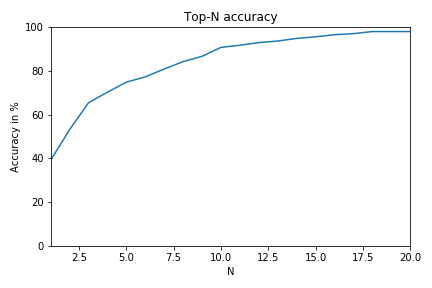
\includegraphics[width=\linewidth]{../figures/top_n_accuracy.png}}
  \caption{Top-N accuracy in percentage}
  \label{fig:topn}
\end{figure}
        \\As we can see, even at its worst, the system is quite good ! There is a $39\%$ chance that the user will pick the first recommended course, a $66\%$ chance that (s)he will pick at least one out of the $3$ first and we reach $90\%$ chances that at least one will be picked out of the total $10$. About precision and recall, here is the graph we obtain at the different top-N levels:
\\\begin{figure}[h]
\centering
\scalebox{0.5}{
  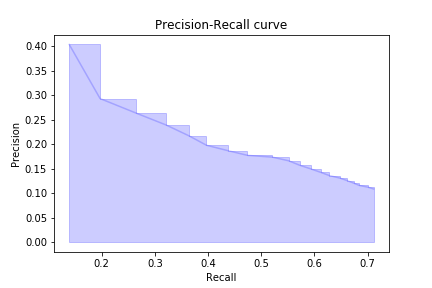
\includegraphics[width=\linewidth]{../figures/precrec.png}}
  \caption{Precision-Recall curve}
  \label{fig:precrec}
\end{figure}

        \newpage
        Obviously since we recommend such a small number of courses, the precision will be lackluster, however we can see a nice trend on the recall which means that out of the ones we recommend, we have a good chunk that the student actually picked !
        \\To get a feel of how many recommendations we should make, here is a graph of the mean average precision at top-N:
\\\begin{figure}[h]
\centering
\scalebox{0.5}{
  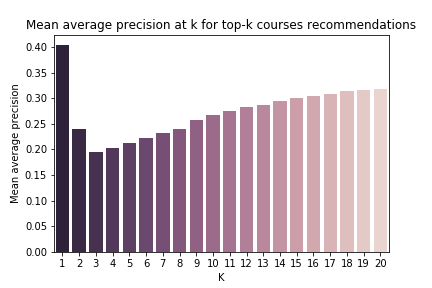
\includegraphics[width=\linewidth]{../figures/mapatk.png}}
  \caption{Mean Average Precision plot}
  \label{fig:mapatk}
\end{figure}
        \\The graph shows that it's pointless to recommend a ton of courses, and we should focus around $3$ to $5$ recommendations, however, we recommend $10$ courses for the demo, to be able to see if the recommendations still make sense after the first few ones.

\newpage
\section{Future Work}
    Building a recommender system for courses is quite a tremendous task, and much is left to be accomplished. Namely, the first thing that comes to mind is the need for a better UI in order to have it up and running on a server at all times for students to try out. Letting students toying around with the system and asking them questions about it could allow us to derive another metric to measure its efficiency. Also, we should quickly focus the attention on the combination of models, as removing the correlation of grades inbetween courses might not affect the results too much, hence, following Occam's razor, there is an argument to be made for it to be dismissed. Of course there are a lot of variables in the school's database that could be leveraged, but the first one we could think about is the years. We could take our focus towards creating a time series-based model that could fit into the pipeline, the idea being that the further back we go in history, the less important registrations should be for example. Another angle is one that we've previously discussed, a graph-based approach. It makes total sense that the students could be clustered together, and to do so, we could use the description of each course, and apply an LDA to them for example. If we find interesting topics, we might be able derive a model out of them.
    \\And last but not least, we could simply ask the student about his/her preferences concerning a few sub-domains and use that information to weigh the scores for each course !

\section{Conclusion}
    In this report, we presented a course recommendation system whose purpose is to recommend EPFL courses to students based on their previously chosen ones or on courses they know that they will enjoy. The system is presented as a proof-of-concept and not as a full-blown production ready software. There is still much left to be done, but with the constant grow of the machine-learning field, we have no doubt that we will be able to achieve a higher top-N accuracy and as a consequence, have a state of the art recommender system.

\newpage
\section{Credits}
    This Masters semester project was offered to me by my supervisors Prof. Patrick Jermann, Francisco Pinto and Kshitij Sharma and exceeded all of my expectations. I would like to thank particularly Francisco and Kshitij for their ongoing help and advices during the whole research and implementation, it would have been hard to come up with such a good system without their help. It was a great pleasure to work with both of them and in the CEDE\cite{cede} lab in general.

\begin{thebibliography}{23}
\bibitem{cdae}
Collaborative Denoising Auto-Encoder,
\\\texttt{http://alicezheng.org/papers/wsdm16-cdae.pdf}

\bibitem{cdaegithub}
Implementation of CDAE,
\\\texttt{https://github.com/henry0312/CDAE}

\bibitem{keras}
Keras library,
\\\texttt{https://github.com/keras-team/keras}

\bibitem{cede}
The CEDE laboratory at EPFL,
\\\texttt{https://moocs.epfl.ch/}

\bibitem{jaccard}
The Jaccard similarity on wikipedia,
\\\texttt{https://en.wikipedia.org/wiki/Jaccard\_index\#Generalized\_Jaccard\_similarity\_and\_distance}

\bibitem{jensen}
The Jensen-Shannon divergence on wikipedia,
\\\texttt{https://en.wikipedia.org/wiki/Jensen\%E2\%80\%93Shannon\_divergence\#Definition}

\end{thebibliography}

\end{document}
